% !TEX root = ../ifvWorkshopQuality.tex
\section{Data Science: Tools and Techniques}
\frame{\frametitle{Tools for Data Scientist}
\framesubtitle{}
\begin{columns}[t] 
     \begin{column}[T]{7cm} 
     	\begin{itemize}
     		\item Programming languages:
		\begin{itemize}
		\item R
		\item Python
		\item SAS
		\item ...
		\end{itemize}
		\item Visualisation app:
		\begin{itemize}
		\item Tableau
		\end{itemize}
		\item Development Environment (IDE):
		\begin{itemize}
		\item Jupyter
		\item Spyder
		\end{itemize}
		\item Also potentially:
		\begin{itemize}
		\item Matlab
		\item Scilab
		\item ...
		\end{itemize}
     	\end{itemize}
  For installation, visit: https://www.anaconda.com/ \\
  Data folder:\\
  http://bit.ly/ifv122019
     \end{column}
     	\begin{column}[T]{7cm} 
         	\begin{center}
            		\includegraphics[width=0.95\textwidth]{Jupyter}\source{}
        		\end{center}
     \end{column}
 \end{columns}
}

\frame{\frametitle{Python Introduction}
	}

\frame{\frametitle{Get started}
\framesubtitle{Create your first jupyter notebook}
\begin{columns}[t] 
     \begin{column}[T]{7cm} 
     	\begin{itemize}
		\item Python 
		\begin{itemize}
			\item is interpreted
			\item can be run on terminal or IDE
		\end{itemize}
		\item Indentation is strict, defines program structures (no braces)
		\item Dynamically typed
		\begin{itemize}
			\item No variable declaration required
		\end{itemize}
		\item Syntax
		\begin{itemize}
			\item Refer to example worksheets
		\end{itemize}
		\item Data structures
		\begin{itemize}
			\item List: \texttt{l = [1, 2, ``a'']}
			\item Tuples: \texttt{t = (1, 2, ``a'')}
			\item Dictionaries: \texttt{d = \{``a'':1, ``b'':2\}}
			\item Sets: \texttt{s = set(\[1, 2, 3, 4\])}
		\end{itemize}
	\end{itemize}
     \end{column}
     	\begin{column}[T]{7cm} 
         	%\begin{center}
            		\StickyNote[5cm]{
			\begin{itemize}
				\item[$\square$] Open a new jupyter notebook
				\item[$\square$] Print ``Hello World''
				\item[$\square$] Run a \texttt{for}-loop
				\begin{itemize}
					\item using \texttt{range(...)}
					\item printing the loop variable
				\end{itemize}
				\item[$\square$] Create an example of the data structures listed
				\item[$\square$] Access their elements
				\end{itemize}}
        		%\end{center}
     \end{column}
 \end{columns}
}

\frame{\frametitle{Pandas Introduction}
\framesubtitle{}
\begin{columns}[t] 
     \begin{column}[T]{7cm} 
     	\begin{itemize}
	\item Pandas is a framework for manipulation and handling of series and rectangular data
	\item Extremely efficient and powerful
	\item Syntax
		\begin{itemize}
			\item \texttt{import pandas as pd}
			\item \texttt{df = pd.DataFrame(...)}
			\item \texttt{df.head()}
			\item \texttt{df[``Column'']}
			\item \texttt{df[df[``Column''] == 0]}	
		\end{itemize}
	\item Data structures:
	\begin{itemize}
		\item Series (\texttt{pd.Series(\textsf{from e.g. array})})
		\item DataFrame (\texttt{pd.DataFrame(\textsf{from e.g. dicts})})
	\end{itemize}
\end{itemize}
     \end{column}
     	\begin{column}[T]{7cm} 
         	\StickyNote[5cm]{
			\begin{itemize}
				\item[$\square$] Import Pandas
				\item[$\square$] Create a DataFrame (\texttt{pd.DataFrame}) from a dictionary
				\item[$\square$] Show the \texttt{head} of the DataFrame 
				\item[$\square$] Show only certain parts of the DataFrame, e.g. all non-zeros entries
			\end{itemize}}
     \end{column}
 \end{columns}
}

\frame{\frametitle{Get to work!}
\framesubtitle{Load and try \texttt{0-Basics.ipynb (http://bit.ly/ifv122019
)} }
\begin{center}
\includegraphics[width = .3\textwidth]{Wagenmeister.png}
\end{center}
}

\frame{\frametitle{Selected Techniques applied in Data Science}
\framesubtitle{}
\begin{itemize}
\item \textbf{Visualisation}
\item Regression: Linear, Logistic
\item \textbf{Density Estimation}
\item Confidence Intervals
\item Test of Hypotheses
\item Pattern Recognition
\item {Time Series}
\item \textbf{Unsupervised Learning (Clustering)}
\item Supervised Learning
\item Decision Trees
\item \textbf{Monte-Carlo-Simulation}
\item Bayesian Statistics
\item \textbf{Principal Component Analysis}
\item \textbf{Support Vector Machines}
\end{itemize}
}

\subsection{Visualisation}
\frame{\frametitle{Visualisation approaches}
\framesubtitle{Likely, you will all know Excel plots - there is much more to it...}
\begin{columns}[t] 
     \begin{column}[T]{6cm} 
     	\begin{itemize}
     		\item Line plot with / w/o confidence
		\item Bar plots (stacked/grouped)
		\item Histogram
		\item Scatter plot
		\begin{itemize}
		\item Blob sizes
		\item Colors
		\end{itemize}
		\item Box whisker
		\item Bubble chart
		\item Geospatial plots
		\item Surface plot
		\item Heat map
		\item Tree map
     	\end{itemize}
     \end{column}
     	\begin{column}[T]{6cm} 
         	\begin{center}
            		\only<1>{\includegraphics[width=0.9\textwidth]{SingularValues}\source{}}
			\only<2>{
			\begin{tikzpicture}[scale = 0.9]
		\begin{axis}[ybar stacked, 
		colormap/bluered,
		ylabel={m EUR/a},
		legend style={at={(0.5,-0.40)},
		anchor=north, legend columns=3},
		symbolic x coords={EMEA, ASEAN, CIS, E. Europe, NAFTA, RoA, W. Europe},
		xtick=data,
		x tick label style={rotate=45,anchor=east},
		title={Urban Vehicle Market Size}]]
		\addplot[fill = RYB1, draw = RYB1!50!black] coordinates
			{(EMEA,.054) (ASEAN,.152) (CIS, .082) (E. Europe, .392) (NAFTA, .563) (RoA, .043) (W. Europe, 1.309)};
		\addplot[fill = RYB2, draw = RYB2!50!black] coordinates
		{(EMEA,.257) (ASEAN,1.638) (CIS, .052) (E. Europe, .215) (NAFTA, 1.131) (RoA, .607) (W. Europe, .661)};
		\addplot[fill = RYB3, draw = RYB3!50!black] coordinates
		{(EMEA,.142) (ASEAN, .094) (CIS, 0) (E. Europe, 0) (NAFTA, .085) (RoA, .151) (W. Europe, .104)};
		\legend{LRV, Metro, APM};
		\end{axis}
		\end{tikzpicture}}
			\only<3>{\includegraphics[width=0.95\textwidth]{MuHist}\source{}}
			\only<4>{\includegraphics[width=0.95\textwidth]{Scatter}\source{}}
		\only<5>{Intentionally left blank}
			\only<6>{\includegraphics[width=0.95\textwidth]{ReichweiteFilm}\source{}}
			\only<7>{\includegraphics[width=0.95\textwidth]{VTPowerConsumption}\source{}}
			\only<8>{\includegraphics[width=0.95\textwidth]{fxfyr}\source{}}
%			\only<9>{\includegraphics[width=0.8\textwidth]{}\source{}}
%			\only<10>{\includegraphics[width=0.8\textwidth]{}\source{}}
        		\end{center}
     \end{column}
 \end{columns}
}

\subsection{Density Estimation}
\frame{\frametitle{Density estimation}
\framesubtitle{Estimate underlying probability density function from observed data}
\begin{columns}[t] 
     \begin{column}[T]{6cm} 
     	\begin{itemize}
     		\item Analysis of distribution properties from sampled data
		\item Fit an appropriate kernel to the samples
     	\end{itemize}
     \end{column}
     	\begin{column}[T]{6cm} 
         	\begin{center}
		\pgfplotsset{compat=newest,
                      tick label style={font=\sansmath\sffamily},
                      axis line style={draw=black!80, line width=0.1875ex},
                      y tick label style={/pgf/number format/fixed},
                      tick style={major tick length=0.0ex},
                      major grid style={thick, dash pattern=on 0pt off 2pt, black!50},
                      height = 6cm
                    }
                    
            		\begin{tikzpicture}[line cap=round, line join=round]
                    \begin{axis}[ymajorgrids, xmajorgrids]
                    \addplot [ybar, domain=0:15, samples=16, fill=blue!50!cyan, draw=none] 
                      (x, {0.6*norm(x, 4, 0.1) + 0.4*norm(x, 12, .05)});
                    \addplot [very thick, draw=orange,  domain=0:15, samples=100, smooth]
                      (x, {0.6*norm(x, 4, 0.1) + 0.4*norm(x, 12, .05) });
                    \end{axis}
                    \end{tikzpicture}
        		\end{center}
     \end{column}
 \end{columns}
}
%\subsection{Time Series}

\frame{\frametitle{Get to work!}
\framesubtitle{Load and try \texttt{1-Visualisation.ipynb}  (http://bit.ly/ifv122019
)}
\begin{center}
\includegraphics[width = .3\textwidth]{Wagenmeister.png}
\end{center}
}

\frame{\frametitle{What is machine learning?}
\framesubtitle{ML is a field of study that gives computers the ability to learn without being explicitly programmed.}
\begin{columns}[t] 
     \begin{column}[T]{7cm} 
     	\begin{itemize}
     		\item Different paradigm:
		\begin{itemize}
		\item Derive rules from observations
		\end{itemize}
		\item Typical procedure:
		\begin{itemize}
		\item \textbf{Train:} Observe set of examples ``training data''
		\item \textbf{Fit:} Infer information of process behind data
		\item \textbf{Test:} Make prediction on unseen data ``Test data''
		\end{itemize}
		\item Variations:
		\begin{itemize}
		\item Supervised learning: provide labels with data
		\item Unsupervised learning: cluster data based on patterns
		\end{itemize}
     	\end{itemize}
     \end{column}
     	\begin{column}[T]{7cm} 
         	\begin{center}
			Traditional approach:
			\vspace{.5cm}
			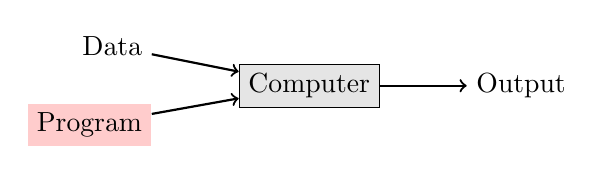
\begin{tikzpicture}
 				\node[anchor = east] (d) at (0,0) {Data};
				\node[anchor = east, fill = red!20] (p) at (0,-1) {Program};
				\node[anchor = west] (o) at (4,-.5) {Output};
				\node[draw, fill = gray!20] (c) at (2,-.5) {Computer};
				\draw[->, thick] (d) -- (c);
				\draw[->, thick] (p)-- (c);
				\draw[->, thick] (c) -- (o);
			\end{tikzpicture}
			
			Machine learning approach:
			\vspace{.5cm}
			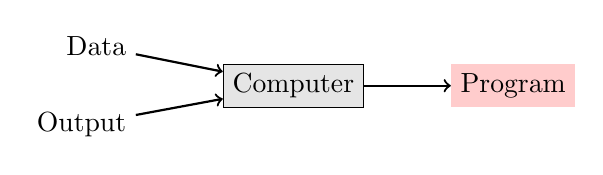
\begin{tikzpicture}
 				\node[anchor = east] (d) at (0,0) {Data};
				\node[anchor = east] (p) at (0,-1) {Output};
				\node[anchor = west,  fill = red!20] (o) at (4,-.5) {Program};
				\node[draw, fill = gray!20] (c) at (2,-.5) {Computer};
				\draw[->, thick] (d) -- (c);
				\draw[->, thick] (p)-- (c);
				\draw[->, thick] (c) -- (o);
			\end{tikzpicture}

		\end{center}
     \end{column}
 \end{columns}
}

\subsection{Unsupervised Learning (Clustering)}
%\frame{\frametitle{Machine Learning}
%\framesubtitle{Using MIT OpenCourseware Slides}
%Source:
%\begin{center}
%Eric Grimson, John Guttag, and Ana Bell. 6.0002 Introduction to Computational Thinking and Data Science. Fall 2016. Massachusetts Institute of Technology: MIT OpenCourseWare, https://ocw.mit.edu. License: Creative Commons BY-NC-SA.
%\end{center}
%}
%\setbeamercolor{background canvas}{bg=}
%%\frame{
%
\includepdf[page = 4-6]{OCW/ML.pdf}%}

\frame{\frametitle{Clustering}
\framesubtitle{Two fundamental approaches, $k$ number of clusters defined \textit{a priori}}
\begin{columns}[t] 
     \begin{column}[T]{7cm} 
     \textbf{Hierarchical clustering}
     	\begin{enumerate}
     		\item Assign each item to one cluster
		\item Find closest (most similar cluster): merge them
		\item Continue until desired number of clusters $k$ is reached
     	\end{enumerate}
     \end{column}
     	\begin{column}[T]{7cm} 
         	\textbf{K-means clustering}
     	\begin{enumerate}
		\item Randomly choose $k$ initial centroids
		\item While centroids don't change
		\begin{enumerate}
		\item[E:] Create $k$ clusters by assigning each item to closest centroid
		\item[M:] Compute $k$ new centroids by averaging items in each cluster
		\end{enumerate}
     	\end{enumerate}
     \end{column}
 \end{columns}
 
\begin{center}
 	\includegraphics[width = .9\textwidth]{expectation-maximization}
\end{center}
}

\frame{\frametitle{K-means clustering procedure}
         	\begin{center}
            		\only<1>{\includegraphics[width=0.7\textwidth]{PCAprocedure0}\source{}}
			\only<2>{\includegraphics[width=0.7\textwidth]{PCAprocedure1}\source{}}
			\only<3>{\includegraphics[width=0.7\textwidth]{PCAprocedure2}\source{}}
			\only<4>{\includegraphics[width=0.7\textwidth]{PCAprocedure3}\source{}}
			\only<5>{\includegraphics[width=0.7\textwidth]{PCAprocedure4}\source{}}
			\only<6>{\includegraphics[width=0.7\textwidth]{PCAprocedure5}\source{}}
			%\only<7>{\includegraphics[width=0.7\textwidth]{PCAprocedure6}\source{}}

        		\end{center}}
		
\frame{\frametitle{K-means inappropriate cluster number}
         	\begin{center}
            		\only<1>{\includegraphics[width=0.7\textwidth]{PCAprocedureFewCluster0}\source{}}
			\only<2>{\includegraphics[width=0.7\textwidth]{PCAprocedureFewCluster1}\source{}}
			\only<3>{\includegraphics[width=0.7\textwidth]{PCAprocedureFewCluster2}\source{}}
			\only<4>{\includegraphics[width=0.7\textwidth]{PCAprocedureFewCluster3}\source{}}
			\only<5>{\includegraphics[width=0.7\textwidth]{PCAprocedureFewCluster4}\source{}}
			\only<6>{\includegraphics[width=0.7\textwidth]{PCAprocedureFewCluster5}\source{}}
			%\only<7>{\includegraphics[width=0.7\textwidth]{PCAprocedure6}\source{}}

        		\end{center}}



\subsection{Principal Component Analysis}
%\frame{\frametitle{Principal Component Analysis (PCA)}
%\framesubtitle{Using MIT OpenCourseware Slides}
%Source:
%\begin{center}
%Philippe Rigollet. 18.650 Statistics for Applications . Fall 2016. Massachusetts Institute of Technology: MIT OpenCourseWare, https://ocw.mit.edu. License: Creative Commons BY-NC-SA.
%\end{center}
%}
%
%\setbeamercolor{background canvas}{bg=}
%%\frame{
%
\includepdf[page = 2-16]{OCW/PCA.pdf}%}

\frame{\frametitle{Principal Component Analysis (PCA)}
\framesubtitle{Reduce dimensionality of data}
\begin{columns}[t] 
     \begin{column}[T]{7cm} 
     	\begin{itemize}
     		\item Sample $X_{1}, \ldots, X_{n}$ is a cloud of points in $\mathbb{R}^d$
		\item Typically, $d$ is large
		\item<1-> \textbf{Question:} can we project the point cloud onto a linear subspace of dimension $d' < d$ while keeping as much of the information as possible?
		\item<2-> \textbf{Answer:} PCA achieves this by keeping important aspects of the covariance structure in orthogonal directions.
     	\end{itemize}
     \end{column}
     	\begin{column}[T]{7cm} 
         	\begin{center}
            		\includegraphics[width=0.6\textwidth]{GaussianScatterPCA}\source{}
        		\end{center}
     \end{column}
 \end{columns}
}



\subsection{Support Vector Machines}

\frame{\frametitle{Support Vector Machine}
\framesubtitle{Separate data into subsets according to their $nD$-coordinates.}
\begin{columns}[t] 
     \begin{column}[T]{5cm} 
     	\begin{itemize}
		\item Idea:
		\begin{itemize}
		\item Find separating hyperplane maximising the distance between borderline instances
		\item For data mixed in feature space, slack parameter (and penalty $C$) is used
		\item If no separating hyperplane can be found in feature space, dimension is increased ``Kernel trick''
		\end{itemize}
     		\item Robust:
		\begin{itemize}
		\item High dimensionality
		\item Small datasets
		\end{itemize}
		\item Simple to complex models
     	\end{itemize}
     \end{column}
     	\begin{column}[T]{7cm} 
         	\begin{center}
		\only<1>{
            		\begin{tikzpicture}[>=stealth', scale = 0.9]
                      % Draw axes
                      \draw [<->,thick] (0,5) node (yaxis) [above] {$y$}
                            |- (5,0) node (xaxis) [right] {$x$};
                      % draw line
                      \draw (0,-1) -- (5,4); % y=x-1
                      \draw[dashed] (-1,0) -- (4,5); % y=x+1
                      \draw[dashed] (2,-1) -- (6,3); % y=x-3
                      % \draw labels
                      \draw (3.5,3) node[rotate=45,font=\small] 
                            {$\mathbf{w}\cdot \mathbf{x} + b = 0$};
                      \draw (2.5,4) node[rotate=45,font=\small] 
                            {$\mathbf{w}\cdot \mathbf{x} + b = 1$};
                      \draw (4.5,2) node[rotate=45,font=\small] 
                            {$\mathbf{w}\cdot \mathbf{x} + b = -1$};
                      % draw distance
                      \draw[dotted] (4,5) -- (6,3);
                      \draw (5.25,4.25) node[rotate=-45] {$\frac{2}{\Vert \mathbf{w} \Vert}$};
                      \draw[dotted] (0,0) -- (0.5,-0.5);
                      \draw (0,-0.5) node[rotate=-45] {$\frac{b}{\Vert \mathbf{w} \Vert}$};
                      \draw[->] (2,1) -- (1.5,1.5);
                      \draw (1.85,1.35) node[rotate=-45] {$\mathbf{w}$};
                      % draw negative dots
                      \fill[red] (0.5,1.5) circle (3pt);
                      \fill[red]   (1.5,2.5)   circle (3pt);
                      \fill[black] (1,2.5)     circle (3pt);
                      \fill[black] (0.75,2)    circle (3pt);
                      \fill[black] (0.6,1.9)   circle (3pt);
                      \fill[black] (0.77, 2.5) circle (3pt);
                      \fill[black] (1.5,3)     circle (3pt);
                      \fill[black] (1.3,3.3)   circle (3pt);
                      \fill[black] (0.6,3.2)   circle (3pt);
                      % draw positive dots
                      \draw[red,thick] (4,1)     circle (3pt); 
                      \draw[red,thick] (3.3,.3)  circle (3pt); 
                      \draw[black]     (4.5,1.2) circle (3pt); 
                      \draw[black]     (4.5,.5)  circle (3pt); 
                      \draw[black]     (3.9,.7)  circle (3pt); 
                      \draw[black]     (5,1)     circle (3pt); 
                      \draw[black]     (3.5,.2)  circle (3pt); 
                      \draw[black]     (4,.3)    circle (3pt); 
                    \end{tikzpicture}}
 %%%%%%%%%%%%%                  
                    \only<2>{
                    \vspace{1cm}
                    \begin{tikzpicture}[>=stealth',x=1cm,y=1cm, scale = .5]
 
                        %draw[color=gray] (0,0) grid (6,6);
                        \draw (0,0) rectangle (6,6);
                        % \draw line
                        \draw[color=red,line width=2pt]
                          (2,6) .. controls (3,5.5) and (3,5) .. 
                          (3,5) .. controls (3,4) and (2,2.5) .. 
                          (2,2) .. controls (2,1) and (2.8,1) .. 
                          (3,1) .. controls (3.5,1) and (3.5,2) .. 
                          (4,2) .. controls (4.5,2) and (6,0) .. 
                          (6,0);
                        % \draw left dashed line
                        \draw[dashed] 
                          (1.5,6) .. controls (2.5,5.5) and (2.5,5) .. 
                          (2.5,5) .. controls (2.5,4) and (1.5,2.5) .. 
                          (1.5,2) .. controls (1.5,.5) and (2.8,.5) .. 
                          (3,.5) .. controls (3.75,.5) and (3.5,1.5) .. 
                          (4,1.5) .. controls (4.5,1.5) and (5.5,0) .. 
                          (5.5,0);
                        % \draw right dashed line
                        \draw[dashed] 
                          (2.5,6) .. controls (3.5,5.5) and (3.5,5) .. 
                          (3.5,5) .. controls (3.5,4) and (2.5,2.5) .. 
                          (2.5,2) .. controls (2.5,1.5) and (2.8,1.5) .. 
                          (3,1.5) .. controls (3.25,1.5) and (3.5,2.5) .. 
                          (4,2.5) .. controls (4.5,2.5) and (6,0.5) .. 
                          (6,0.5);
                        %\draw[color=gray] (2,6) -- (3,5) -- (2,2) -- (3,1) -- (4,2) -- (6,0);
                        %\draw[color=gray] (1.5,6) -- (2.5,5) -- (1.5,2) -- (3,.5)-- (4,1.5)-- (5.5,0);
                        %\draw[color=gray] (2.5,6) -- (3.5,5) -- (2.5,2) -- (3,1.5)-- (4,2.5)-- (6,0.5);
                         
                        %\draw[color=gray] (7,0) grid (13,6);
                        \draw (7,0) rectangle (13,6);
                        % \draw line
                        \draw[color=red,line width=2pt] (8.5,6) -- (12,0);
                        % \draw dashed line
                        \draw[dashed]  (8,6) -- (11.5,0);
                        \draw[dashed]  (9,6) -- (12.5,0);
                         
                        \draw[->,thick] (5,3) -- (8,3) node [above,pos=.5] {$\phi$};
                         
                        \def\positive{{%
                        {2.3,5.3},
                        {3.5,.7},
                        {1.5,2},
                        {1.2,2.1},
                        {1.8,.8},
                        {1,5.5},
                        {1.2,5.8},
                        {.75,.2},
                        {2,4},
                        {5, 0.5},
                        {1.5,3},
                        {2.3,.5},
                        %
                        {9.3,3.3},
                        {11,.8},
                        {8.5,2},
                        {7.2,4.1},
                        {8.8,.8},
                        {8,5.5},
                        {8.2,5},
                        {7.75,.2},
                        {9,4.2},
                        {12, 0.5},
                        {8.5,3},
                        {9.3,.5},
                        }}
                         
                        % \draw positive dots
                        \foreach \i in {0,...,20} {
                          \pgfmathparse{\positive[\i][0]}\let \x \pgfmathresult;
                          \pgfmathparse{\positive[\i][1]}\let \y \pgfmathresult;
                          \fill[black] (\x,\y) circle (2pt);
                        }
                         
                        \def\negative{{%
                        {4,2.5},
                        {3.5,5},
                        {2.6,1.6},
                        {4.5,5.2},
                        {5.5,3.7},
                        {3.9,4.7},
                        {5,2.7},
                        {3.5,4.2},
                        {5.8,.9},
                        %
                        {10.75,3},
                        {10.5,5},
                        {11.6,1.6},
                        {11.5,5.2},
                        {12.5,3.7},
                        {10.9,4.7},
                        {12,2.7},
                        {10.5,4.2},
                        {12.8,.9},
                        }}
                         
                        % \draw negative dots
                        \foreach \i in {0,...,16} {
                          \pgfmathparse{\negative[\i][0]}\let \x \pgfmathresult;
                          \pgfmathparse{\negative[\i][1]}\let \y \pgfmathresult;
                          \draw[black] (\x,\y) circle (3pt);
                        }
                         
                        \end{tikzpicture}
                    }
        		\end{center}
     \end{column}
 \end{columns}
}

%\subsection{Further Outlook}

\subsection{Monte-Carlo-Simulation}
\frame{\frametitle{Monte-Carlo-Simulation (MC-Simulation)}
\framesubtitle{}
\begin{itemize}
\item Method of estimating value of unknown quantity using inferential statistics
\item Inferential statistics terms:
\begin{itemize}
		\item Population: set of examples
		\item Sample: Proper subset of population
\end{itemize}
\item Random sample tends to exhibit same properties as population it is drawn from
\end{itemize}
\begin{example}[Flip coins]
 Let's estimate the probabilities of heads vs. tails for an infinite number of coin flips:
 \begin{itemize}
		\item One flip (heads): 100\% heads? 
		\item Two flips (h, h): still 100 \% heads? Confidence level?
		\item 100 flips (52 h, 48 t): Probability of next coin coming up heads 52/100.
		\end{itemize}
\end{example}
}

\frame{\frametitle{Key aspects to be asked in MC-Simulations}
\framesubtitle{}
\begin{itemize}
\item Never possible to guarantee perfect accuracy through sampling
\item Never assume that an estimate is precisely correct
\item How many samples do we need to look at before we can have justified confidence in our answers?
\begin{itemize}
	\item Answer depends on underlying distribution
	\item Especially hard for defects ``Rare event simulation''
\end{itemize}
\end{itemize}
}

\subsubsection{Monte-Carlo-Simulation Application Example}
\frame{\frametitle{MC-Simulation application example: Braking curve}
\framesubtitle{CCS systems rely on braking curves to describe the train's braking capability.}
\begin{columns}[t] 
     \begin{column}[T]{6cm} 
     	\begin{itemize}
     		\item To supervise train velocity, CCS systems predict the future braking capability of the train
		\item However, there is not \textit{the} braking capability
		\item Braking curves exhibit a randomised behaviour
     	\end{itemize}
     \end{column}
     	\begin{column}[T]{6cm} 
         	\begin{center}
			\includegraphics[width=\textwidth]{brakingcurvesND}
        		\end{center}
     \end{column}
 \end{columns}
}

% \frame{\frametitle{White Box Modelling of the braking system}
% \framesubtitle{Which parameters can be identified and which effect do they have on the braking distance?}
% \begin{itemize}
% \item Brake pipe: propagation velocity, flow resistances, train length
% \item Distributor valve: Filling time, brake cylinder pressure
% \item Braking force generation: efficiency, brake radius (for disc brakes), pad/block friction coefficient
% \item Wheel/rail contact: rail surface, contaminants, slip, ...
% \end{itemize}
% \begin{center}
% \begin{center}
%           \includegraphics[width=\textwidth]{TrainBPDiagram}
% \end{center}
% \end{center}
% \begin{itemize}
% 	\item Also discrete failure events need to be considered 
% \end{itemize}
% }

% \frame{\frametitle{Why chose MC-Simulation? What are the challenges?}
% \framesubtitle{}
% \begin{itemize}
% \item Error-propagation:
% \begin{itemize}
% 		\item Conservative: assumes normal distribution for all parameters
% 		\item Complex: requires explicit function formulation and partial differentiation
% \end{itemize}
% \item (Standard) Monte-Carlo-Simulation:
% \begin{itemize}
% 		\item Efficient (in terms of confidence): returns shortest (also asymmetric) confidence interval
% 		\item Inefficient (in terms of computational effort):
% 		\begin{itemize}
% 		\item For rare event $\varepsilon \ll 1$, $N \approx \frac{100}{\varepsilon}$ trials required
% 		\item Typical according to CSM: $\varepsilon \in \left[10^{-7} \ldots  10^{-9}\right] \, \Rightarrow \, N \approx 10^{11}$
% 		\end{itemize}
% \end{itemize}
% \item ERA proposes to precalculate braking curves for limited number of train formations
% \begin{itemize}
% 		\item Freight trains to be handled using braked weight and correction factor
% 		\end{itemize}
% \end{itemize}
% }

% \frame{\frametitle{Importance sampling for MC-Simulations}
% \framesubtitle{Importance sampling (IS) increases the probability of ``desired'' outcomes in Monte-Carlo-Simulations.}
% \begin{itemize}
% \item Typical IS approaches:
% \begin{itemize}
% 		\item Stratification: select only relevant strata of the sampling range
% 		\item Scaling: Scale random variable
% 		\item Translation: Move random variable to more relevant part of sampling space
% 		\item Change of random variable: Replace random variable by one more likely to produce outcomes in the relevant range
% 		\item Adaptive approaches
% 		\end{itemize}
% \item Effect: higher number of samples in region of interest
% \item Correction factor: Likelihood ratio $L(y) = \frac{f(y)}{\tilde{f}(y)}$
% \end{itemize}
% }

% \frame{\frametitle{Application of IS to braking curves}
% \framesubtitle{Select relevant variables for IS.}
% \begin{center}
% \includegraphics[width = .9\textwidth]{mhist}
% \end{center}
% }

% \frame{\frametitle{Application of IS to braking curves}
% \framesubtitle{Change identified random variables, in the case at hand $\mu_{B}$}
% \begin{center}
% \includegraphics[width = .9\textwidth]{BChist}
% \end{center}
% }

% \frame{\frametitle{Application of IS to braking curves}
% \framesubtitle{Analyse for rare events, here braking distances in excess of 1100 m. $N = 5 \cdot 10^7$}
% \only<1>{\begin{center}
% \includegraphics[width = .9\textwidth]{rare}
% \end{center}}
% \only<2>{
% %\hspace{-.62cm}
% \begin{tabular}{|c|c|c|c|c|c|c|}
% \hline
% $s$ & $n_{\mathcal{U}}$ & $p_{\mathcal{U}}$ & $n_{IS, 1}$ & $p_{IS, 1}$ & $n_{IS, 2}$ & $p_{IS, 2}$ \\ \hline
% 1000 & 24400 & 4.89$\cdot 10^{-3}$ & 2.27$\cdot 10^6$ & 1.14$\cdot 10^{-2}$ & 3.11$\cdot 10^5$ & 1.77$\cdot 10^{-3}$ \\ \hline
% 1050 & 2 & 4$\cdot 10^{-7}$ & 6.66$\cdot 10^4$ & 2.02$\cdot 10^{-4}$ & 1.48$\cdot 10^4$ & 1.59$\cdot 10^{-4}$ \\ \hline
% 1100 & 0 & 0 & 115 & 2.04$\cdot 10^{-7}$ & 419 & 7.50$\cdot 10^{-6}$ \\ \hline
% 1150 & 0 & 0 & 0 & 0 & 15 & 3.88$\cdot 10^{-7}$ \\ \hline
% 1160 & 0 & 0 & 0 & 0 & 7 & 2.05$\cdot 10^{-7}$ \\ \hline
% 1170 & 0 & 0 & 0 & 0 & 5 & 1.46$\cdot 10^{-7}$ \\ \hline
% 1180 & 0 & 0 & 0 & 0 & 4 & 1.16$\cdot 10^{-7}$ \\ \hline
% 1190 & 0 & 0 & 0 & 0 & 1 & 2.90$\cdot 10^{-8}$ \\ \hline
% \end{tabular}
% }
% }

\subsection{Practical hints}
\frame{\frametitle{Practical hints for application of data science methods}
\framesubtitle{}
\begin{columns}[t] 
     \begin{column}[T]{6cm} 
     	\begin{itemize}
     		\item Get to know your data
		\item Use training and validation sets
		\item For clustering and ML: 
		\begin{itemize}
		\item Regularise
		\item Remove outliers, NaN
		\end{itemize} 
		\item When building models:
		\begin{itemize}
		\item Don't expect perfect fit
		\item Inspect confusion matrix
		\end{itemize}
     	\end{itemize}
     \end{column}
     	\begin{column}[T]{6cm} 
         	\begin{center}
            		\renewcommand\arraystretch{1.5}
                            \setlength\tabcolsep{0pt}
                            \begin{tabular}{c >{\bfseries}r @{\hspace{0.7em}}c @{\hspace{0.4em}}c @{\hspace{0.7em}}l}
                              \multirow{10}{*}{\parbox{1.1cm}{\bfseries\raggedleft actual\\ value}} & 
                                & \multicolumn{2}{c}{\bfseries Prediction outcome} & \\
                              & & \bfseries p & \bfseries n & \bfseries total \\
                              & p$'$ & \MyBox{True}{Positive} & \MyBox{False}{Negative} & P$'$ \\[2.4em]
                              & n$'$ & \MyBox{False}{Positive} & \MyBox{True}{Negative} & N$'$ \\
                              & total & P & N &
                            \end{tabular}        		
                            \end{center}
     \end{column}
 \end{columns}
}

\frame{\frametitle{Get to work!}
\framesubtitle{Load and try \texttt{2-Container-SVM.ipynb}  (http://bit.ly/ifv122019
)}
\begin{center}
\includegraphics[width = .3\textwidth]{Wagenmeister.png}
\end{center}
}

